\documentclass[a4paper,12pt]{article}
\usepackage[T1]{fontenc}
\usepackage[utf8]{inputenc}
\usepackage{graphicx}
\usepackage{amsmath}
\usepackage{amsfonts}
\usepackage{amssymb}
\usepackage{booktabs}
\usepackage{float}
\usepackage{geometry}
\usepackage[german]{babel}
\usepackage{enumitem}
\usepackage{parskip}
\usepackage{underscore}
\usepackage{hyperref}
\usepackage{icomma}
% \usepackage{multicol}

\geometry{a4paper, left=25mm, right=25mm, top=20mm, bottom=20mm}

%%%%%%%%%%%%%%% Titelblatt %%%%%%%%%%%%%%%
\begin{document}
\begin{titlepage}
    \centering
    
\includegraphics[scale = 0.03]{bilder/JKU_Logo.png}\\[1.0 cm]	% JKU Logo
    \textsc{\Large Einführungspraktikum Physik}\\[0.5 cm]	        % LVA Name
    \textsc{\large 3. Versuch}\\[0.5 cm]				            % Versuch Nummer    // [x] TODO: Versuch Nummer anpassen
    \rule{\linewidth}{0.4 mm} \\[0.4 cm]
    { \huge \bfseries Brennweite}\\                                 % Versuch Name      // [x] TODO: Versuch Name anpassen
    \rule{\linewidth}{0.4 mm} \\[1.5 cm]
    \begin{minipage}{0.8\textwidth}
        \begin{flushleft} \large
            \emph{Autoren:}\\
            Eva Brandstätter (k12406599)\\
            Tobias Mittermair (k12412801)\\
            \vspace{1cm}
            \emph{Gruppe:}\\
            Freitag Vormittag\\
            \vspace{1cm}
            \emph{Betreuer:}\\
            Gerald Gmachmeir
        \end{flushleft}
        \begin{flushright} \large
            \vspace{8cm}
            \emph{Abgabe:} \\
            \today
        \end{flushright}
    \end{minipage}~    
\end{titlepage}

%%%%%%%%%%%%%%% Inhaltsverzeichnis %%%%%%%%%%%%%%%
\tableofcontents
\newpage


%%%%%%%%%%%%%%% Inhalt %%%%%%%%%%%%%%%
\section{Einleitung}
%//[ ] TODO: Einleitung
% Was soll gemessen werden? (Ziel / Motivation / Hypothese / erwartetes Ergebnis)

In diesem Versuch soll die Brennweite und die zugehörige Unsicherheit einer Sammellinse durch 
das Bessel-Verfahren bestimmt werden.

\section{Grundlagen}
%//[ ] TODO: Grundlagen
% (kurz!) Was muss ich über die zu messende Größe wissen?

% Größe s beschreiben (Bezug auf optische bank)
<>

\section{Versuchsbeschreibung}
\subsection{Versuchsaufbau}
%//[ ] TODO: Versuchsaufbau
% Wie sieht der Versuchsaufbau aus? (Skizze, Anleitung, Geräte, …)
% auf Abbildungen Bezug nehmen

Der Versuch wurde am 13.12.2024 im Praktikumsraum P122 an der JKU in Linz zwischen 11:15 und
13:15 durchgeführt.

Für diesen Versuch wurden eine Sammellinse, ein Lineal, eine optische Bank (mit Reitern, LED
mit Kondensorlinse, Geodreieck als Objekt und Schirm) bereitgestellt.
Weiters stand ein Laptop zur Führung des Laborprotokolls bereit und zur Dokumentation der Werte.
In der nachstehenden Abbildung \ref{Abb:Versuchsaufbau1} ist der Aufbau des Versuches dargestellt.
Dabei ist zu erkennen, dass von links weg eine LED mit Kondensorlinse, danach der Objektträger
mit Geodreieck und darauffolgend eine Linse, vor dem sich ganz rechts befindenden Schirm auf der
optischen Bank angeordnet sind.

% Bild vom Versuchsaufbau
\begin{figure}[H]
    \centering
    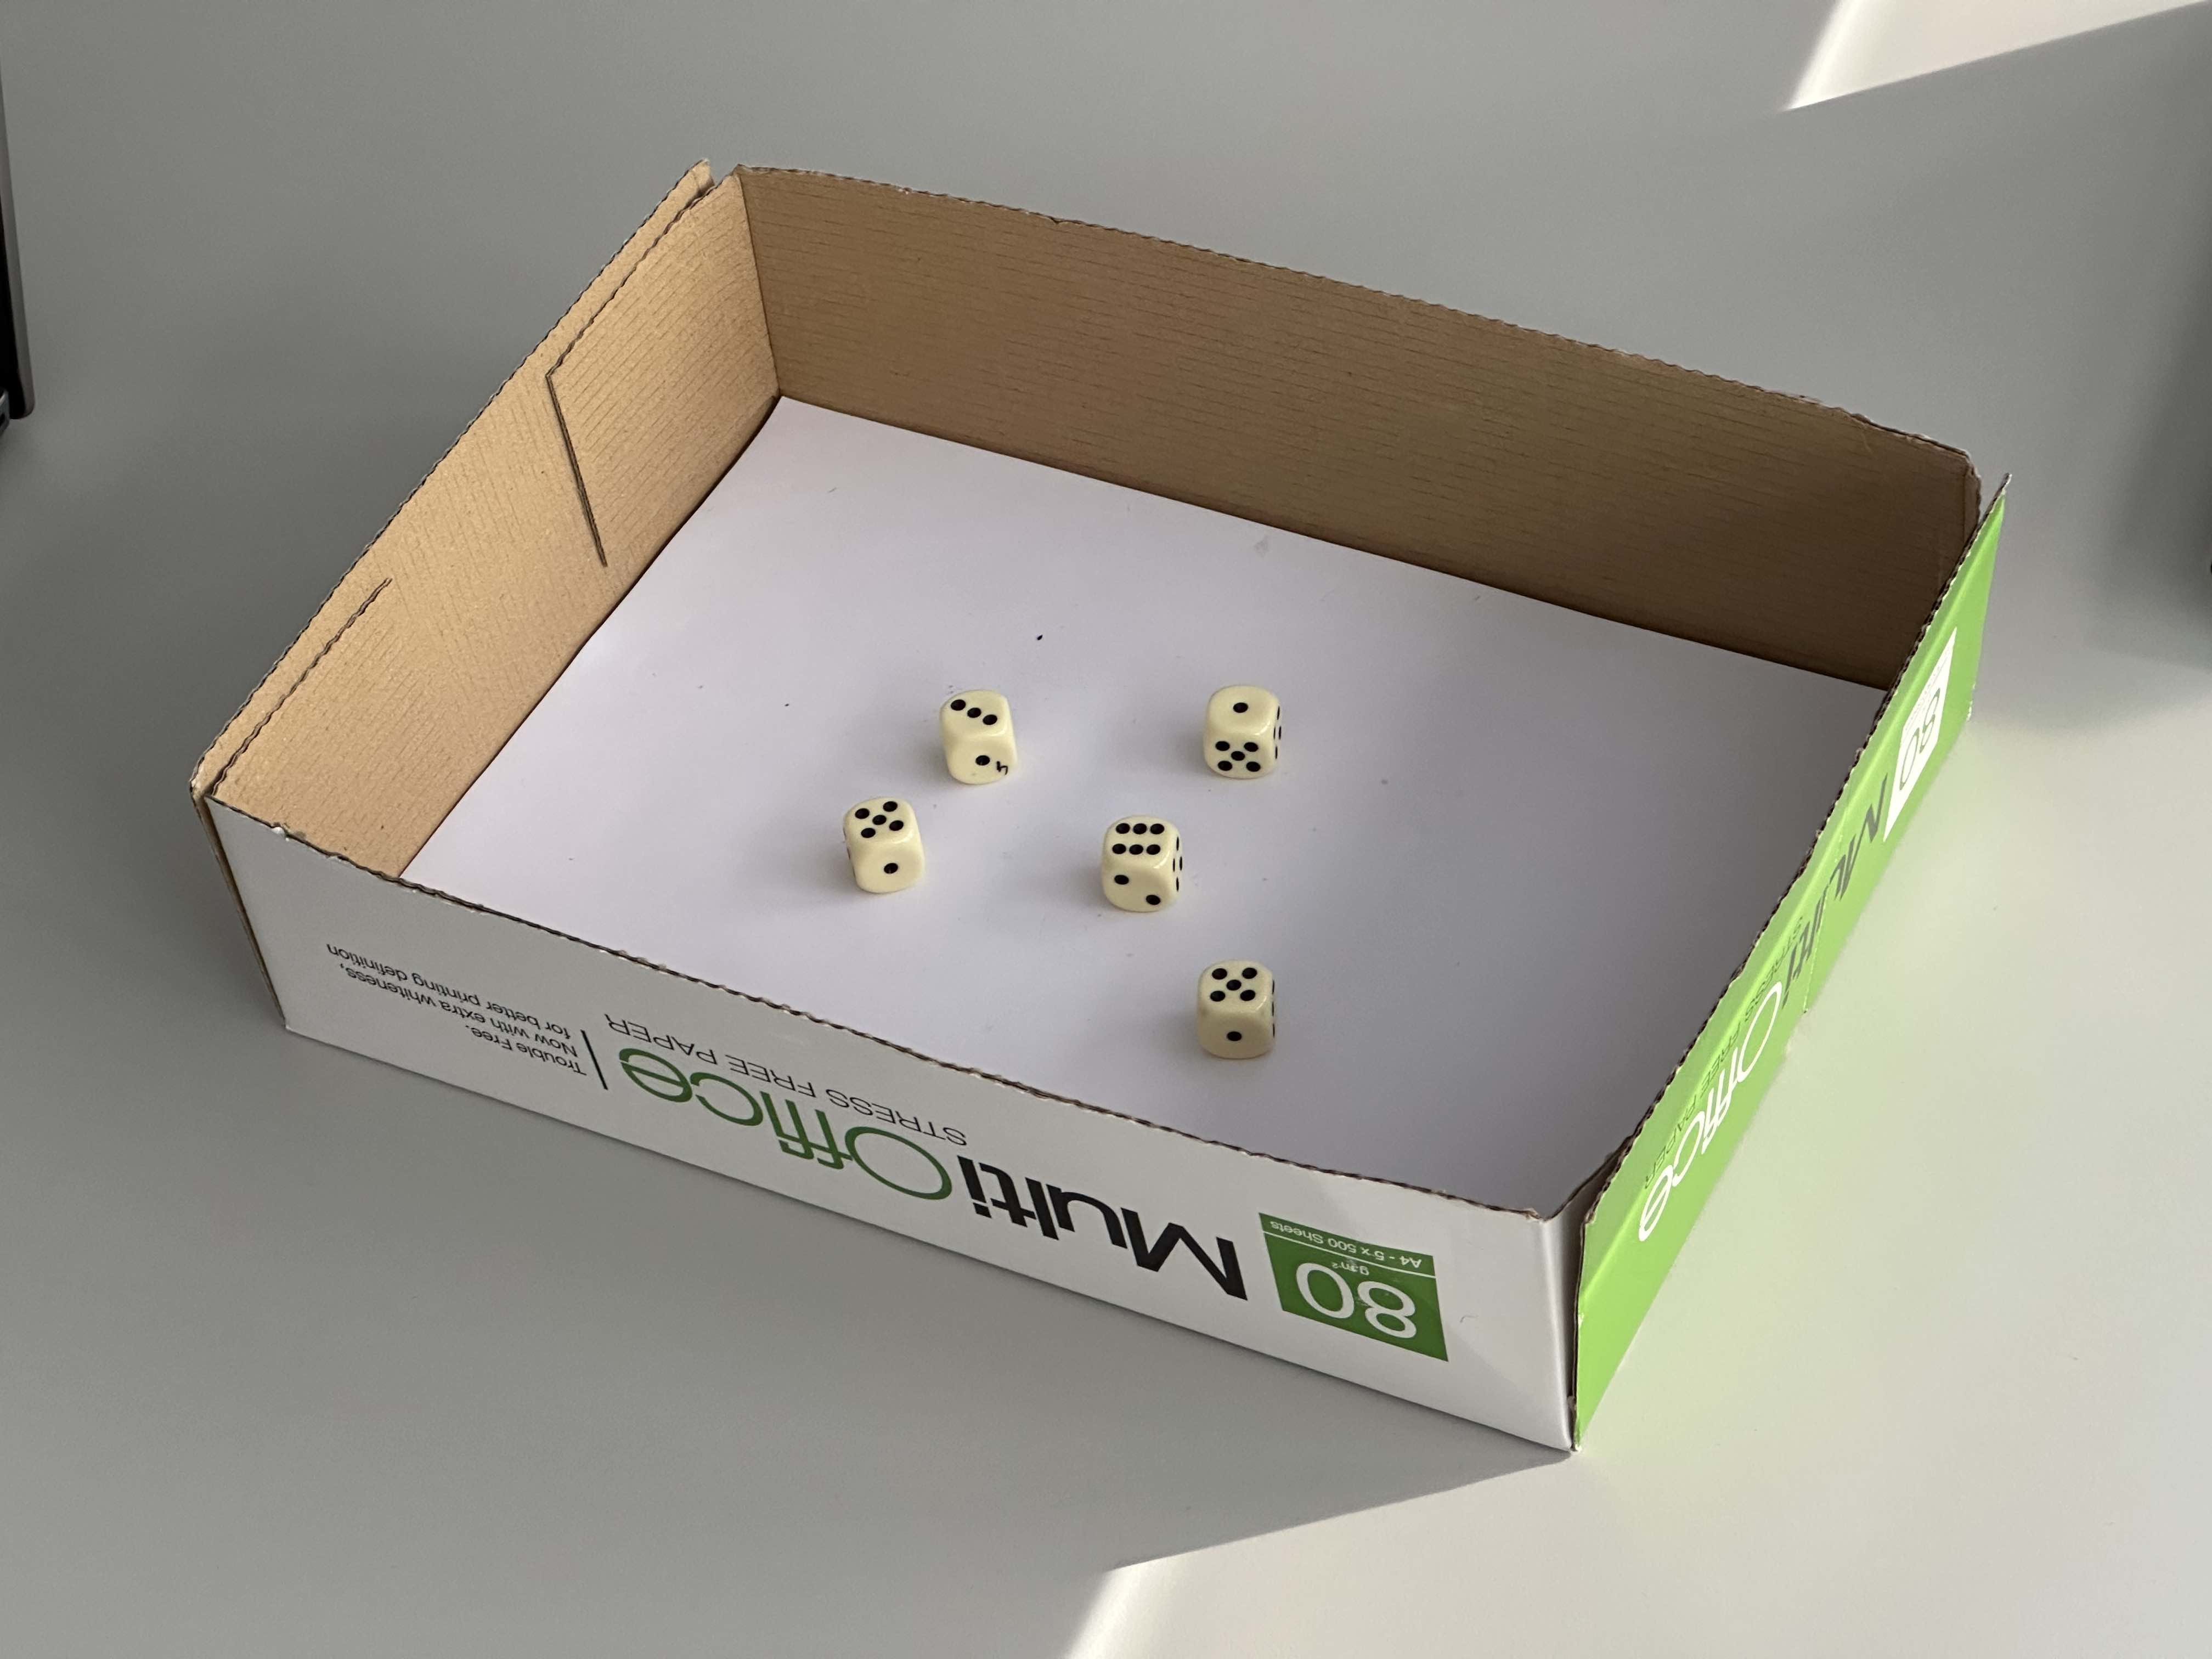
\includegraphics[width=0.5\textwidth]{bilder/Versuchsaufbau1.jpg}           %// [x] TODO: Versuchsaufbau Bild anpassen
    \caption{optische Bank mit optischen Elementen}                             %// [x] TODO: Versuchsaufbau Bildunterschrift anpassen
    \label{Abb:Versuchsaufbau1}
\end{figure}

\subsection{Durchführung}
%//[ ] TODO: Durchführung
% Wie wurde der Versuch durchgeführt bzw. ausgewertet?
% auch wann und wo?

Vor dem tatsächlichen Versuch wurde zuerst die Brennweite der Linse grob abgeschätzt.
Dabei wurde die Linse über den Labortisch gehalten und so lange auf und ab bewegt, bis das
Abbild der Deckenbeleuchtung scharf erkennbar war. Der Abstand zwischen Linse und Abbildung
wurde dann mit dem Lineal abgemessen. Dieser Abstand entspricht annähernd der Brennweite
der Linse und beträgt ungefähr 9,6cm $\pm\:1\mathrm{cm}$. Dies kann man sagen, da der Abstand
zur Deckenleuchte im Verhältnis zum Abstand der Abbildung zur Linse hinreichend groß ist.

Nun kann mit dem eigentlichen Versuch begonnen werden, da jetzt $s>4f$ gewählt werden kann.
Somit wählt man das erste $s$ und stellt den Abstand zwischen Gegenstand und Schirm auf der
optischen Bank ein. Nun wird die Linse so verschoben, dass sich auf dem Schirm ein scharfes
Abbild des Gegenstandes einstellt. Symmetrisch zum mittelpunkt von $s$ ist die zweite Position,
an der die Linse auch ein scharfes Bild erzeugt. 


\section{Messergebnisse und Auswertung}
%//[ ] TODO: Messung - evtl. nur Verweis auf Messergebnisse
% Eigentliche Messung!
% Wie groß sind die Messunsicherheiten („Messfehler“)?

Die Messwerte sind dem auf \url{https://eln.jku.at/} zugänglichen bzw. dem angehängten Laborprotokoll unter \ref{Anhang} zu entnehmen.         %//[x] TODO: Protokoll Dateiname anpassen

%//[ ] TODO: Auswertung
% evtl. Formeln, etc.
% auf richtiges Runden der Werte achten
% evtl. auf Gleichungen Bezug nehmen

\begin{equation}
    \label{Gl1}
    x = x
\end{equation}

\vspace{0,5cm}


% Diagramm(e) der Auswertung
\begin{figure}[H]
    \label{AbbAuswertung1}
    \centering
    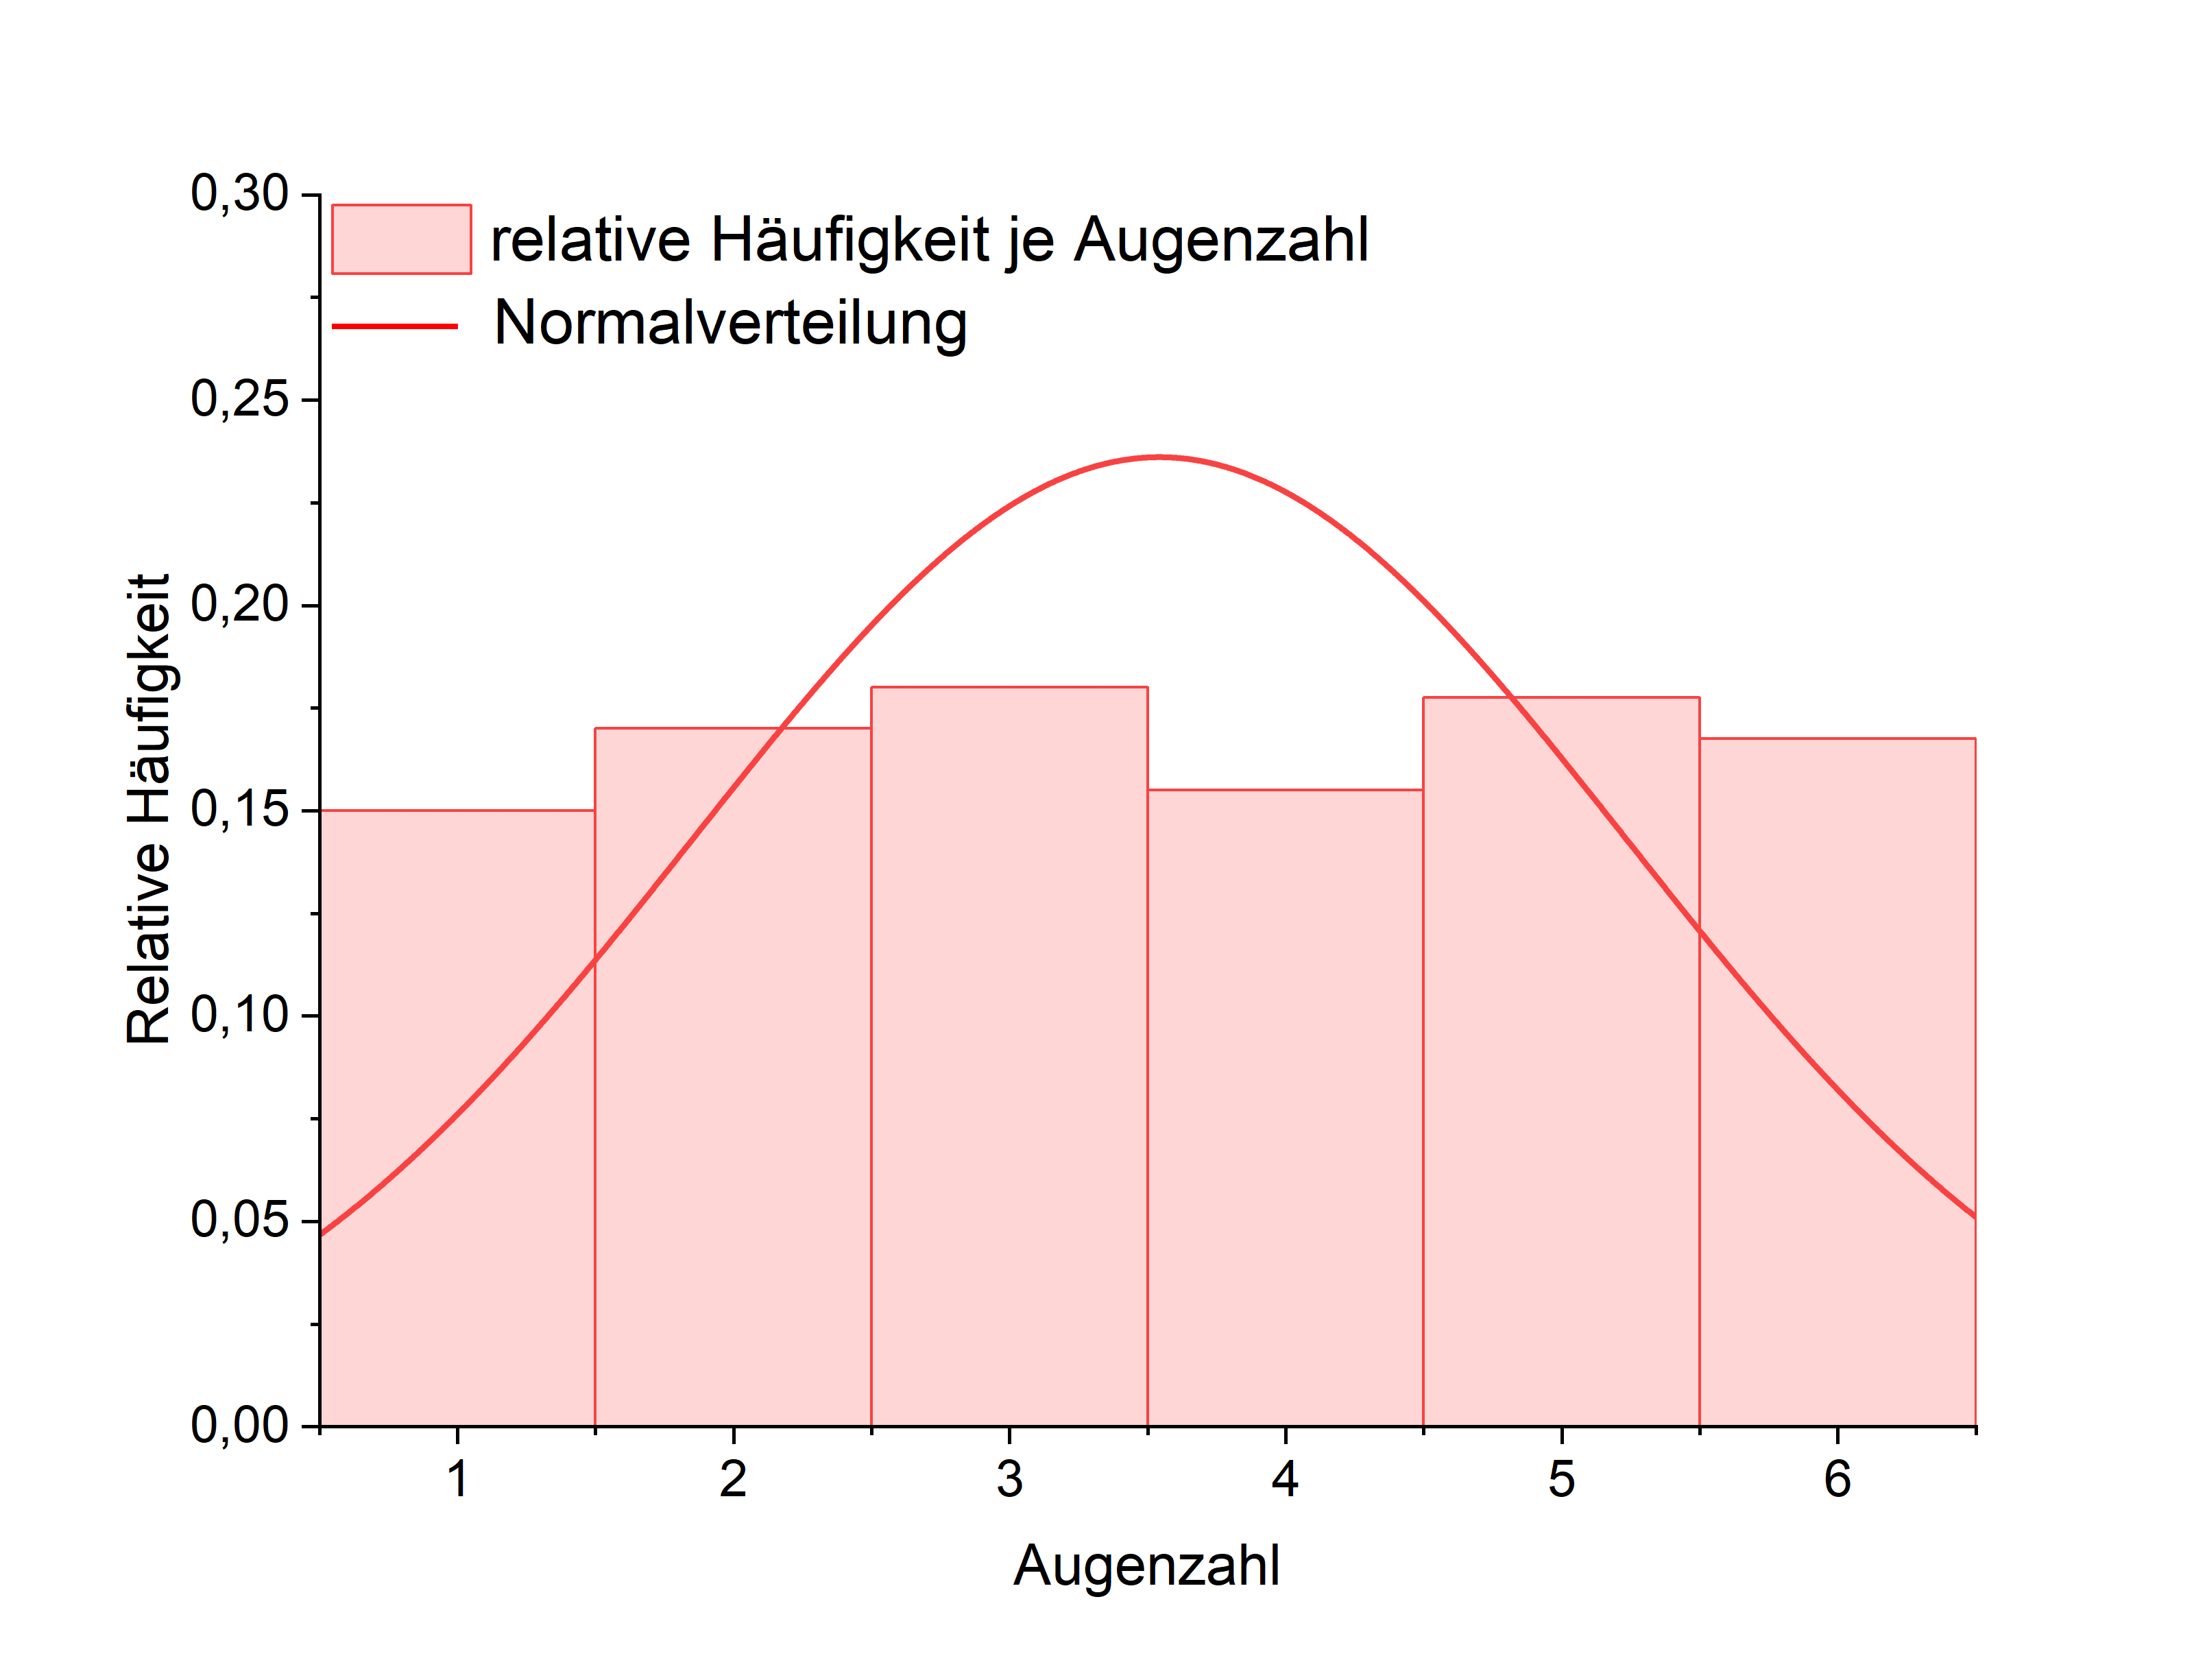
\includegraphics[width=\textwidth]{bilder/Diagramm1.png}        %// [ ] TODO: Diagramm Bild anpassen
    \caption{<>}                                                    %// [ ] TODO: Diagramm Bildunterschrift anpassen
\end{figure}

\section{Diskussion}
%//[ ] TODO: Diskussion
% Wie vergleicht sich meine Messung mit anderen Messungen/Theorien?
% Ist der Messwert sinnvoll? Stimmt die Größenordnung?
% Wo wurden Fehler gemacht? Was kann man verbessern?
% Gegebenenfalls rekursiv auswerten oder nachmessen!
% ursprüngliche Fragestellung diskutieren
% zB Standardabweichung diskutieren, berechnete Größen nennen

<>

\section{Anhang}
\label{sec:Anhang}

\end{document}
